\chapter{Atchweliad Logistaidd}\label{cha:Atchweliad_logistaidd}
\section{Cefndir}
Defnyddiwn atchweliad logistaidd i fodelu'r tebygolrwydd o ddosbarthu gwrthrych i mewn i setiau deuaidd. Mae'n ddull o ddysgu dan oruchwyliaeth sy'n cael ei ddefnyddio yn aml yn academ\"{i}au a diwydiannau. Gall y atchweliad cael ei ddefnyddio i weld os mae rhywun yn curo/colli, s\^{a}l/iachus neu basio/methu mewn rhyw sefyllfa benodol. Gall y syniad yma cael ei ymestyn, gall wahanol atchweliadau logistaidd cael ei rhoi yn baralel i geisio rhoi'r tebygolrwydd o liw llygaid rhyw berson er enghraifft. Mewn termau mwy cyffredinol, gall ymestyn atchweliadau logistaidd i weithio ar setiau o labeli di-deuaidd. O hyn ymlaen fyddem yn edrych ar atchweliadau gyda labeli deuaidd. 

Mae'n hawdd delweddu sut fydd atchweliad logistaidd gydag un newidyn annibynnol. Gwelwn fod y model yn edrych fel y graff yn ddarlun~\ref{fig:Enghraifft_o_atchweliad_logistaidd} pan hyn yw'r sefyllfa.

\begin{figure}[H]
\begin{center}
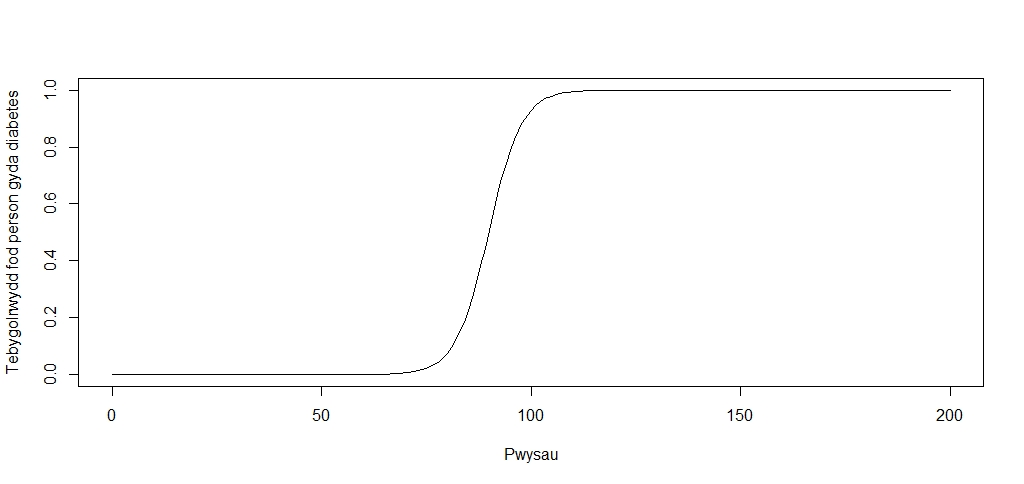
\includegraphics[width=0.5\linewidth]{../img/Atchweliad_logistaidd.jpeg}
\label{fig:Enghraifft_o_atchweliad_logistaidd}
\caption{Enghraiff o atchweliad logistaidd.}
\end{center}
\end{figure}

Gwelwn yn y graff nesaf fod y plot yn dangos ein data mewn ffordd rhesymol os wnawn gymharu i y cyfrannau o'r pwyntiau yn pob un o'r adrannau. Gwelwn y cyfrannau o phob adran yn glas yn ffigwr~\ref{fig:Enghraifft_o_atchweliad_logistaidd_pwyntiau}. 

\begin{figure}[H]
\begin{center}
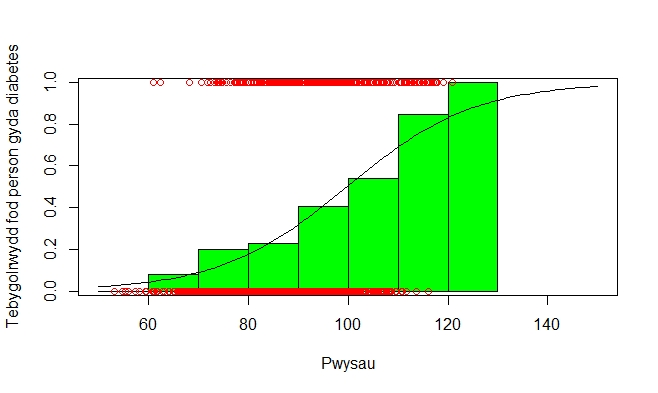
\includegraphics[width=0.5\linewidth]{../img/atchweliad_logistaidd_gyda_pwyntiau.jpeg}
\label{fig:Enghraifft_o_atchweliad_logistaidd_pwyntiau}
\caption{Enghraiff o atchweliad logistaidd gyda labelau.}
\end{center}
\end{figure}

Os wnawn cymharu y model logistaidd i model llinol, er fod yn bosib cael model gwell yn llinol, mae'n bwysig gwybod pa parth mae'r model angen cael cynhaliad ynddo. Gwelwn yn y plot yn ffigwr~\ref{fig:Enghraifft_o_atchweliad_llinol} fod dydi y model ddim yn cynnal cynhaliad ar gyfer mewnbwn llai na $60$ a fwy na $120$ gan fod y tebygolrwydd yn anniffiniedig (Hynny yw, dydi ddim yn bosib cael $P(\mathbf{x})<0$ a $P(\mathbf{x})>1$). 

\begin{figure}[H]
\begin{center}
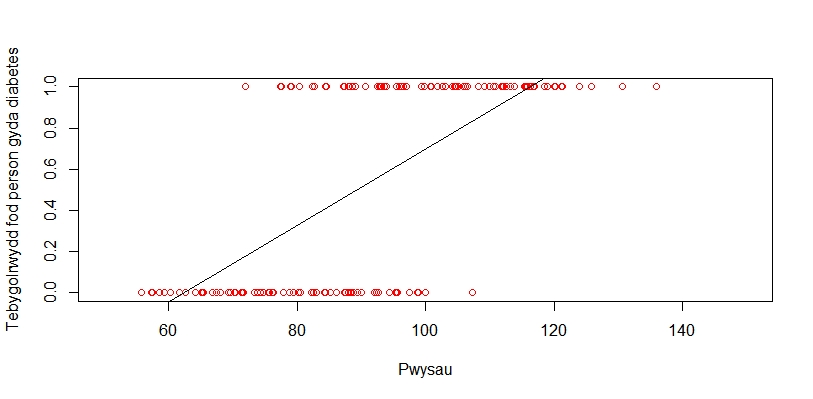
\includegraphics[width=0.5\linewidth]{../img/cymharu_llinol.jpeg}
\label{fig:Enghraifft_o_atchweliad_llinol}
\caption{Enghraiff o atchweliad llinol i ein data.}
\end{center}
\end{figure}

\section{Sut mae atchweliad logistaidd yn gweithio?}

Wnawn ddiffinio'r fector sy'n cynnwys gwybodaeth am berson $j$ ($j \in {1,\dots,n}$) gyda $\mathbf{x}_j$ sydd hefo dimensiwn o $m$ (hynny yw bod yna $m$ priodweddau). Yn ogystal, wnawn ddiffinio $y_j$ fel label deuaidd i berson $j$, yr hyn rydyn ni eisiau rhagfynegi. Yna gydag ein data fydd rhaid i ni wahanu'r data i mewn i ddata ymarfer ac ddata profi. Fydd hyn yn cael ei wneud ar hap. Felly fydd gennym:

Data ymarfer: $\mathbf{x}_j$ a $y_j$ ar gyfer $j \in \{ 1,\dots,k\}$ lle mae $k<n$

Data profi: $\mathbf{x}_j$ a $y_j$ ar gyfer $j \in \{ k+1,\dots,n \}$

Nawr wnawn edrych ar y ffwythiant logistaidd, lle mae $z \in (-\infty,\infty)$:

\begin{equation}\label{eqn:gwrthdrologit}	
	f(z) = \frac{1}{1+e^{-z}} 
\end{equation}

Mae'r model logistaidd yn cymryd y gwrthdro o ffurf logit, mae hyn yn cael ei ddangos yn hafaliad~\ref{eqn:gwrthrologit}.

\begin{equation}\label{eqn:cyfernodau} 
    z = \alpha + \beta_{1}X_{1} + \dots + \beta_{m}X_{m} 
\end{equation} 

Felly mae hafaliad~~\ref{eqn:modellog} yn dangos y model cyfan.

\begin{equation}\label{eqn:modellog}
    P(\mathbf{x}) = P(y = 1 | x_1 \dots x_k) = \frac{1}{1+e^{-( \alpha + \sum_{i=1}^{m} \beta_{i}x_{i})}} 
\end{equation}

\subsection{Yr Algorithm}
\cite{Logistic-regression}
Fydd $\alpha$ a $\mathbf{\beta}$ y paramedrau fyddem yn trio amcangyfrif o wybod $\mathbf{x}$ ac $y$ y data ymarfer. I amcangyfrif hyn wnawn ddefnyddio'r dull amcangyfrif tebygoliaeth fwyaf. Cymerwn $\hat{\mathbf{z}}$ i fod y fector o baramedrau fyddem yn amcangyfrif. Yna mae gennym y amcangyfrif tebygoliaeth ganlynol a fyddem yn trio cael y gwerth agosaf i $1$. 

\begin{equation}\label{eqn:amcangyfrif}
L(\hat{\mathbf{z}}) = \prod_{s \in y_{i}=1} p(x_i) \prod_{s \in y_{i}=0} (1 - p(x_i))
\end{equation}

Mae Hafaliad~\ref{eqn:amcangyfrif} yn trio uchafsymio y lluoswm o phob tebygolrwydd ag oedd yn edrych ar labeli y data ymarfer. Gan fod rhai labeli am fod yn $0$ a rydym yn lluosi y rhifau yma, mae rhaid newid y dechneg ag lluoswm y tebygolrwydd $(1 - p(x_i))$ i phob $i$ sydd gyda'r label $0$ i alluogi trio darganfod y paramedrau sy'n creu yr uchafswm (yn ein sefyllfa ni fydd yr uchafswm y rhif agosaf tuag at $1$). 

Sydd yn gallu cael ei symleiddio i:

$$ L(\hat{\mathbf{z}}) = \prod_{i=1}^{k} p(x_i)^{y_i} (1 - p(x_i))^{1-y_i} $$

Nawr fyddem yn cymryd y log o'r amcangyfrif tebygoliaeth.

$$ \log L(\hat{\mathbf{z}}) = \sum_{i=1}^{n} y_{i} \log(p(x_{i})) + (1-y_{i}) \log(1-p(x_{i})) $$

Sydd yn symleiddio i:

$$ \log L(\hat{\mathbf{z}}) = \sum_{i=1}^{n} y_{i} \log \left(\frac{1}{1 + e^{-\hat{\mathbf{z}}\mathbf{x}}} \right) + (1 - y_i) \log \left(\frac{e^{-\hat{\mathbf{z}}\mathbf{x}}}{1 + e^{-\hat{\mathbf{z}}\mathbf{x}}} \right) $$

ac felly:

$$ \log L(\hat{\mathbf{z}}) = \sum_{i=1}^{n} y_i \hat{\mathbf{z}} x_i - \log(1 + e^{\hat{\mathbf{z}} x_i}) $$

Yna mae gennym y log o'r amcangyfrif tebygoliaeth. Rydym eisiau darganfod y gwerth o $z$ lle mae'r log o'r amcangyfrif tebygoliaeth ar ei fwyaf.

$$ \hat{\mathbf{z}} = \arg \max_{\mathbf{z}} \log L(\mathbf{z})  $$

Does yna ddim ffordd bendant o ddatrys yr hafaliad uchod, fydd angen defnyddio algorithmau fel swm lleiaf sgwariau wedi eu hail bwyso drwy iteriadau neu ddisgyniad fwyaf fel gwelwn yn y algorithmau yn R ac Python yn y drefn honno. 

Mae'r dull disgyniad fwyaf yn algorithm optimeiddiaeth trefn cyntaf i darganfod isafbwynt lleol o ffwythiant gall ei ddifferu. Mae'r algorithm yn cymryd camau yn gyfraneddol ir graddiant yn y pwynt yno. Fydd yr algorithm am phob cam yn edrych yn debyg i hafaliad~\ref{eqn:disgyniadfwyaf} gyda $a$ yn rhyw bwynt a $f$ yn y ffwythiant.

\begin{equation}\label{eqn:disgyniadfwyaf}
  a_{n+1} = a_{n} - \nabla f
\end{equation}

Ar gyfer y swm lleiaf o sgwariau wedi eu hail bwyso drwy iteriadau, mae'r algorithm yn cydgyfeirio tuag at y pwysau optimaidd ar gyfer y cyfernodau yn Fformiwla~\ref{eqn:cyfernodau}. Mae angen ail bwyso oherwydd mae'r amrywiant yn newid trwy gydol y model. Mae lle mae'r amrywiant ar ei fwyaf yn y model am dynodi lle fydd gromlin ein model.

Unwaith mae gennym amcangyfrif o'r paramedrau, mae angen darganfod pa mor dda yw ein model logistaidd. I wneud hwn byddwn yn rhoi ein data profi $x_j$ i mewn i'r model, a cynharu'r allbwn gyda $y_j$. Fel allbwn cawn tebygolrywdd, rhif rhwng $0$ ac $1$, yna wnawn talgrynnu'r allbwn i cael label. Wedyn mae gennym ein rhagfynegiad am label pob person, yna gallwn ddarganfod cyfradd llwyddiant ein model gan:

$$ 1 - \sum_{j = k+1}^{n} \frac{(P(\mathbf{x}_j) - y_j)^{2}}{n - k} $$

Mae'r swm yma yn cymryd y canran o camgymeriadau rhwng y data ymarfer a'r data profi ac yna yn ei tynnu i ffwrdd o $1$, darganwyd hyn y cyfradd llwyddiant. I darganfod y canran o camgymeriadau fyddwn yn tynnu y data profi oddiwrth y data ymarfer, ac yno yn sgwario yr matrics canlyniadol. Fydd y gweithrediadau yma yn gweithio yn \^{o}l elfen. Unwaith fydd y matrics wedi'i sgwario fydd pob elfen sy'n dangos $1$ yn dangos camgymeriad ac felly fydd $0$ yn dangos rhagfynegiad cywir. Yna fydd y matrics yn cael ei symio ac fydd y cyfanswm yn cael ei rhannu gan y nifer o elfennau.

\section{Tiwtorial yn R}

Yn yr enghraifft hon, fyddwn yn edrych ar ddata ar 1000 o bobol, fydd y data yn cynnwys gwybodaeth ar uchder, pwysau, maint gwasg, oed, rhyw ag oes gan y person diabetes. Mae'n bosib lawrlwytho'r data oddi yma: \url{https://dysgupeirianyddol.github.io/}

Ar gyfer gwneud atchweliad logistaidd, mae angen y pecyn \mintinline{R}{stats} a wnawn ei lawrlwytho a'i gosod gan redeg y canlynol:

\begin{minted}[bgcolor=green!7]{r}
> install.packages("stats")
> library(stats)
\end{minted}

Yna fydd rhaid lwytho'r data i mewn a'i arbed fel newidyn. Fydd rhaid neud yn si\^{w}r fod y ffwythiant \mintinline{R}{read.csv} yn cael ei chyfeirio tuag at y lleoliad cywir o le mae eich data chi wedi'i gadw.

\begin{minted}[bgcolor=green!7]{r}
> data <- read.csv("C:/Users/User/Desktop/Dysgu_Peirianyddol/data_logistic.csv")
\end{minted}

Unwaith ei fod ar ein consol, mae'n bosib gweld y data:

\begin{minted}[bgcolor=green!7]{r}
> View(data)
\end{minted}

\begin{figure}[H]
\begin{center}
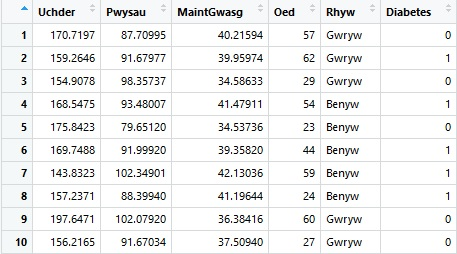
\includegraphics[width=0.5\linewidth]{../img/data_diabetes_r.jpg}
\end{center}
\end{figure}

Nawr wnawn rannu'r data fel bod $70\%$ o'r data yw'r data ymarfer ac $30\%$ o'r data yw'r data profi. Fyddwn yn rhannu'r data ar hap. 

\begin{minted}[bgcolor=green!7]{r}
> rhifau <- c(1:1000)
> rhifauymarfer <- sample(x = rhifau, size = 700, replace = FALSE)
> rhifauprofi <- setdiff(rhifau, rhifauymarfer)
\end{minted}

Mae'r c\^{o}d uchod yn rhannu'r setiau gan ddefnyddio eu indecs (rhif y rhes) yn y data ac yno mae'r c\^{o}d isod yn rhannu'r fectorau i mewn i setiau arwahan. 

\begin{minted}[bgcolor=green!7]{r}
> ymarfer <- data[rhifauymarfer,] 
> profi <- data[rhifauprofi,]
\end{minted}

Nawr rydym yn barod i greu'r model logistaidd. I greu'r model fyddem yn rhedeg y c\^{o}d gan ddefnyddio y ffwythiant \mintinline{R}{glm}, sydd yn fyr am "Generalized Linear Models", sydd yn golygu gall y ffwythiant cael ei ddefnyddio am lawer fwy o atchweliadau na logistaidd yn unig. Oherwydd hyn mae angen gosod yr opsiwn \mintinline{R}{family} i \mintinline{R}{binomial}. I ddilyn strwythur o'r algorithm, byddwn yn creu'r model o'r data ymarfer yn unig. 

\begin{minted}[bgcolor=green!7]{r}
> atchweliad <- glm(Diabetes ~ Uchder + Pwysau + Oed + Rhyw + MaintGwasg,
+                   family = binomial,
+                   data = ymarfer)
\end{minted}

Unwaith mae'r model wedi'i greu, gallwn weld eu paramedrau sydd wedi cael ei amcangyfrif:

\begin{minted}[bgcolor=green!7]{r}
> atchweliad$coefficients
 (Intercept)       Uchder       Pwysau          Oed 
22.858432583 -0.254347133  0.215272873  0.057360113 
   RhywGwryw   MaintGwasg 
-8.074052403 -0.003206262 
\end{minted}

Felly mae'r model sydd gennym, i dri lle degl, yn edrych fel:

$$ P(\mathbf{x}) = \frac{1}{1 + e^{-22.858 + 0.254 x_{\text{Uchder}} - 0.215 x_{\text{Pwysau}} - 0.057 x_{\text{Oed}} + 8.074 x_{\text{Rhyw}} + 0.003 x_{\text{MaintGwasg}}}} $$

Gan fod ein model wedi'i chwblhau, gallwn weld sut mae'n perfformio yn penderfynu os oes gan bobl y set profi diabetes ta ddim. Geith hyn ei wneud yn defnyddio'r ffwythiant \mintinline{R}{predict} a dewis yr opsiwn \mintinline{R}{type} fel "response" i gael allbwn o debygolrwydd. Heb wneud hyn, fydd yr allbwn yn cyfrifo $z$ o hafaliad~\ref{eqn:cyfernodau}. 

\begin{minted}[bgcolor=green!7]{r}
> canlyniad <- predict(object = atchweliad, newdata = profi, type = "response")
> canlyniad <- round(canlyniad, digits = 0)
> canlyniad <- unname(canlyniad)
\end{minted}

Fyddem yn ogystal yn talgrynnu'r tebygolrwydd o bob person i cael dewis ar os gennym ddiabetes ta ddim. Wedyn fyddem yn tynnu i ffwrdd y rhifau o'r rhesi ar y fector o labeli. Nawr gennym y rhagfynegiad a'r canlyniadau gwreiddiol, gallwn gyfrifo'r canran o'r ddau set sy'n debyg. Gallwn gyfrifo yn y ffurf ganlynol gan fod ein setiau yn ddeuaidd:

\begin{minted}[bgcolor=green!7]{r}
> 1-(sum((test[,6]-unname(canlyniad))**2)/length(test[,6]))
0.8833333
\end{minted}

Fel y gwelwn, mae ein model gydag effeithiolrwydd o $88\%$ ar gyfer y data sydd gennym. Gallwn ni defnyddio y model rydym wedi creu i benderfynu ar os gan berson newydd ar hap diabetes neu ddim. Gwelwn hyn gan gyflwyno dyn gydag uchder o 160, pwysau 92, maint gwasg o 34 ag ugain oed yn y c\^{o}d isod: 

\begin{minted}[bgcolor=green!7]{r}
> unname(round(predict(object = atchweliad, 
+                      newdata = data.frame(Uchder = 160,
+                                           Pwysau = 92, 
+                                           MaintGwasg = 34, 
+                                           Oed = 20, 
+                                           Rhyw = "Gwryw"), 
+                      type = "response"),
+              digits = 0))
+ 
0
\end{minted}

Am y person yma gwelwn fod y model wedi rhagfynegu nad oes ganddo diabetes. Os wnawn ystyried person gyda'r un nodweddion ond yn fenyw:

\begin{minted}[bgcolor=green!7]{r}
> unname(round(predict(object = atchweliad,
+                      newdata = data.frame(Uchder = 160,
+                                           Pwysau = 92, 
+                                           MaintGwasg = 34, 
+                                           Oed = 20, 
+                                           Rhyw = "Benyw"), 
+                      type = "response"),
+              digits = 0))
+ 
1
\end{minted}

Gwelwn fod y model yn rhagfynegi ei fod hi gyda diabetes.

\section{Tiwtorial yn Python}

Ar gyfer cynhyrchu atchweliad logistaidd yn python mae rhaid i ni ddefnyddio'r pecynnau \mintinline{python}{sklearn}, a \mintinline{python}{pandas} i trin y dada. Wnawn lwytho'r pecynnau gan redeg y c\^{o}d yma:

\begin{minted}[bgcolor=cyan!7]{python}
>>> from sklearn.linear_model import LogisticRegression
>>> import pandas as pd
\end{minted}

Nawr mae angen llwytho'r data, wnawn ddefnyddio'r un data wnaethom ddefnyddio i'r tiwtorial yn R. Cewch ei lawrlwytho o .... Mae'n cynnwys 1000 o cofnodion data ar fesuriadau pobl yn cynnwys uchder, pwysau, maintgwasg, oed, rhyw ag label yn dangos os gan y person diabetes neu ddim.  

\begin{minted}[bgcolor=cyan!7]{python}
>>> data = pd.read_csv('data_logistic.csv')
\end{minted}

Gallwn gweld yr data gan rhedeg:

\begin{minted}[bgcolor=cyan!7]{python}
>>> data.head()
\end{minted}

\begin{figure}[H]
\begin{center}
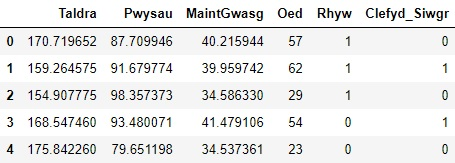
\includegraphics[width=0.5\linewidth]{../img/data_diabetes_python.jpg}
\end{center}
\end{figure}

Gan fod ein data gyda rhyw wedi cael ei diffinio gyda'r geiriau ``Gwryw'' a ``Benyw'', mae python yn cael trafferth yn delio gyda nhw. Felly nawn trawsnewid nhw i newidyn deuaidd (set o $1$ a $0$).

\begin{minted}[bgcolor=cyan!7]{python}
>>> data['Rhyw'] = data['Rhyw'].apply(lambda x: int(x =='Gwryw'))
\end{minted}

Nawr fydd rhaid i ni rannu'r data i ddata ymarfer ag data profi.

\begin{minted}[bgcolor=cyan!7]{python}
>>> ymarfer = data.sample(frac = 0.7)
>>> profi = data.drop(ymarfer.index)
\end{minted}

Mae'r wybodaeth rydym angen i greu model logistaidd angen fod yn fatrics yn python, felly:

\begin{minted}[bgcolor=cyan!7]{python}
>>> X = ymarfer[['Uchder', 'Pwysau', 'MaintGwasg', 'Oed', 'Rhyw']].as_matrix()
>>> y = ymarfer['Diabetes'].as_matrix()
>>> X_profi = profi[['Uchder', 'Pwysau', 'MaintGwasg', 'Oed', 'Rhyw']].as_matrix()
>>> y_profi = profi['Diabetes'].as_matrix()
\end{minted}

I redeg yr atchweliad logistaidd wnawn ddefnyddio'r ffwythiant yn \mintinline{python}{sklearn}. Wnawn wneud gan redeg y c\^{o}d canlynol:

\begin{minted}[bgcolor=cyan!7]{python}
>>> clf = LogisticRegression(random_state=0).fit(X, y)
\end{minted}

Gallwn edrych ar y rhyngdoriad gan

\begin{minted}[bgcolor=cyan!7]{python}
>>> clf.intercept_
array([ 1.70933553])
\end{minted}

ac yna y paramedrau eraill:

\begin{minted}[bgcolor=cyan!7]{python}
>>> clf.coef_
array([[-0.12384414,  0.14710498,  0.12995053,  0.04682347, -4.80795833]])
\end{minted}

Felly dyma yw ein model i dri lle degol:

$$ P(\mathbf{x}) = \frac{1}{1 + e^{-1.709 + 0.124 x_{\text{Uchder}} + 0.147 x_{\text{Pwysau}} - 0.047 x_{\text{Oed}} + 4.808 x_{\text{Rhyw}} - 0.130 x_{\text{MaintGwasg}}}} $$

Nawr gallwn ni cyfrifo'r gyfradd llwyddiant o ein model ar y data profi. Gallwn ei chyfrifo yn y ffordd ganlynol oherwydd ein bod yn delio gyda data deuaidd.

\begin{minted}[bgcolor=cyan!7]{python}
>>> 1-(sum((clf.predict(X_profi)-y_profi)**2)/len(y_profi))
0.91666666666666663
\end{minted}

Felly mae ein model logistaidd yn python yn rhoi cyfradd llwyddiant o tua $92\%$. Gallwn nawr ei ddefnyddio ar gyfer rhyw berson tu allan i ein data. Os oes gennym wryw gyda thaldra o 171, pwysau o 130 a maint gwasg ag oed o 40; gallwn ragfynegi os oes gan y person diabetes ta ddim. 

\begin{minted}[bgcolor=cyan!7]{python}
>>> clf.predict([[171, 130, 40, 40, 1]])
array([1], dtype=int64)
\end{minted}

Gwelwn fod y model logistaidd yn rhagfynegu bod gan y person hwn diabetes. Nawr nawn drio gyda person tebyg ond gyda phwysau o 90 yn lle.

\begin{minted}[bgcolor=cyan!7]{python}
>>> clf.predict([[171, 90, 40, 40,1]])
array([0], dtype=int64)
\end{minted}

Gwelwn nad oes gan y person yma diabetes.